\documentclass{article}
\usepackage[utf8]{inputenc}
\usepackage{authblk}
\title{Testing Particle Swarm Optimization Parameters Using Griewank Function}
\author{Alejandro Reyes}
\affil{\it{University of Texas Rio Grande Valley}\\ \it{Statistical Methods PHYS 5394}}
\date{April 2021}

\usepackage{natbib}
\usepackage{graphicx}


\begin{document}

\maketitle

\section{Introduction}
Based on the movement of bird flocks, Particle Swarm Optimization (PSO) is a method which can be used to maximize the value of a function by iteratively testing candidate parameter locations and improving their value relative to their neighbors \cite{wiki:pso}.
This report showcases a series of tests ran on a PSO method script \cite{git:sdm} to optimize the parameters of an n-dimensional Griewank benchmark function \cite{ieee:standard}.

\subsection{Software and Specifications}
All computational methods have been performed using Matlab r2020b release on a machine with specifications listed in table \ref{table:specs}.

\begin{table}[h]
\centering
\begin{tabular}{ | c | c | }
\hline
     Operating System & Ubuntu 20.04.2 \\
\hline
     CPU & Intel i7-9750H 2.60GHz \\
\hline
     Clock speed & 833 Mhz, 4500 Mhz max \\
\hline
     Cores & 6 \\
\hline
     RAM & 15.5 Gb \\
\hline
\end{tabular}
\caption{Machine specifications.}
\label{table:specs}
\end{table}

\subsection{The Griewank Function}

I chose to test the PSO algorithm to minimize the coordinates of the generalized Griewank function (\ref{eq:griewank}) in 30 dimensions for its complexity.
When plotted in 2 dimensions (see figure \ref{eq:griewank}), it is saturated with local minima and is more jagged when compared to the Rastrigin function \cite{ieee:standard}.
The Griewank function has a global minimum equal to 0 at the origin in D dimensions.

\begin{equation}
f = \frac{1}{4000}\sum_{i}^{D}x_{i}^{2}-\prod_{i=1}^{D}\cos(\frac{x_{i}}{\sqrt{i}})+1
\label{eq:griewank}
\end{equation}

\begin{figure}[h!]
\centering
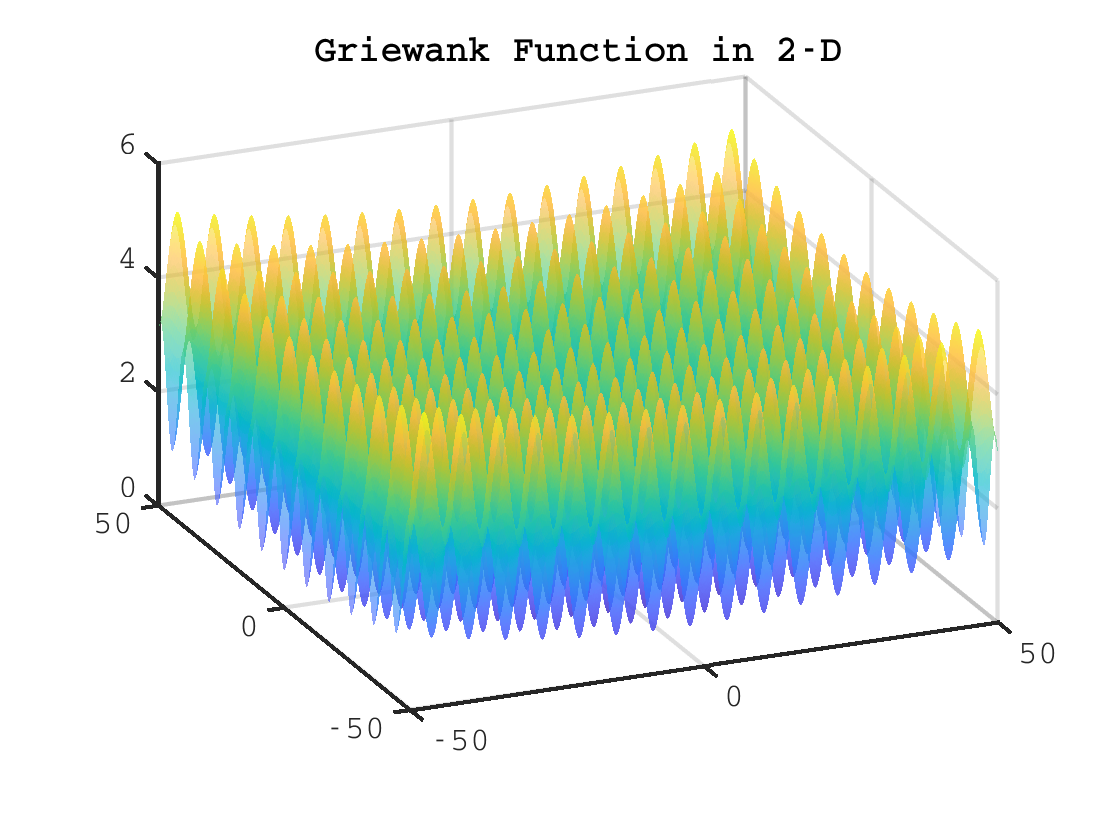
\includegraphics[width=0.8\textwidth]{griewank_3d}
\caption{Griewank function in 2 dimensions.}
\label{fig:griewank}
\end{figure}

\section{Test Runs}

I individually tested the number of trials, particles, and steps and layed out my results in the following subsections.

\subsection{Number of Trials}

First, it is necessary to find an appropriate number of trials which will yield precise parameter coordinates before focusing on accuracy.
I used the default arguments of \textit{crcbpso.m} of 40 particles and 2000 steps and compared the best fitness values across multiple runs, each run corresponding to a different number of trials. 
I also retrieved the average fitness value and the standard deviation of each run.
17 runs were executed ranging from 6 to 180 trials.
I set my experiment this way predicting that the standard deviation should go down as we increase the number of trials.

\begin{figure}[h!]
\centering
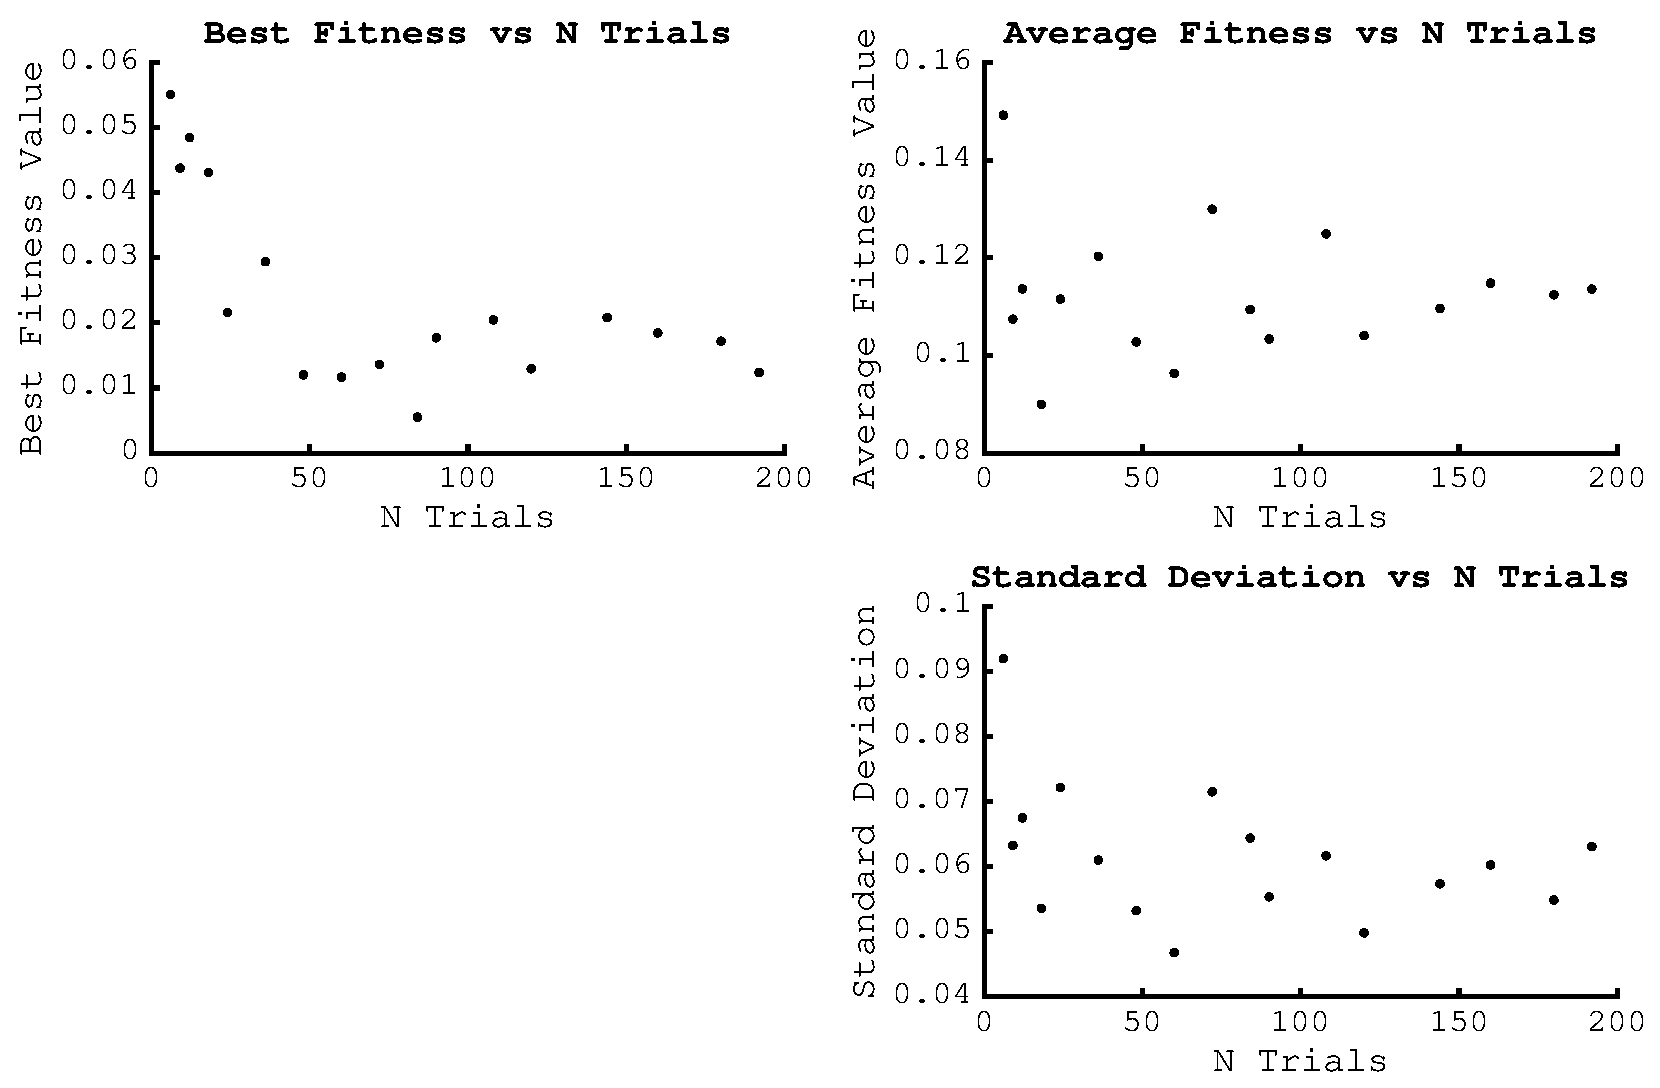
\includegraphics[width=0.8\textwidth]{trials_fig1}
\caption{Best fitness, average, and standard deviation for various runs of varying number of trials.}
\label{fig:trials_1}
\end{figure}

Visual inspection of plots in figure \ref{fig:trials_1} shows the average fitness narrowing down on a value as the number of trials is increased.
As predicted, standard deviation seems to decrease and stabilize.
Furthermore, the best fitness value approaches the correct minimum of 0 before it plateaus close to 72 runs.

The computation time ranged from 2.37 s at 6 trials (or less), to 72.23 s at 180 trials according to the Matlab Profiler tool.
Time increased by a factor of 0.4 s per trial added.
This test was performed using 6 cores (6 workers) in parallel.
I tried enabling multithreading with Parallel Computing Toolbox, however I learned that this would only get two Matlab processes to share the same physical core and compete for computation time.

\subsection{Number of Particles}

\begin{figure}[h!]
\centering
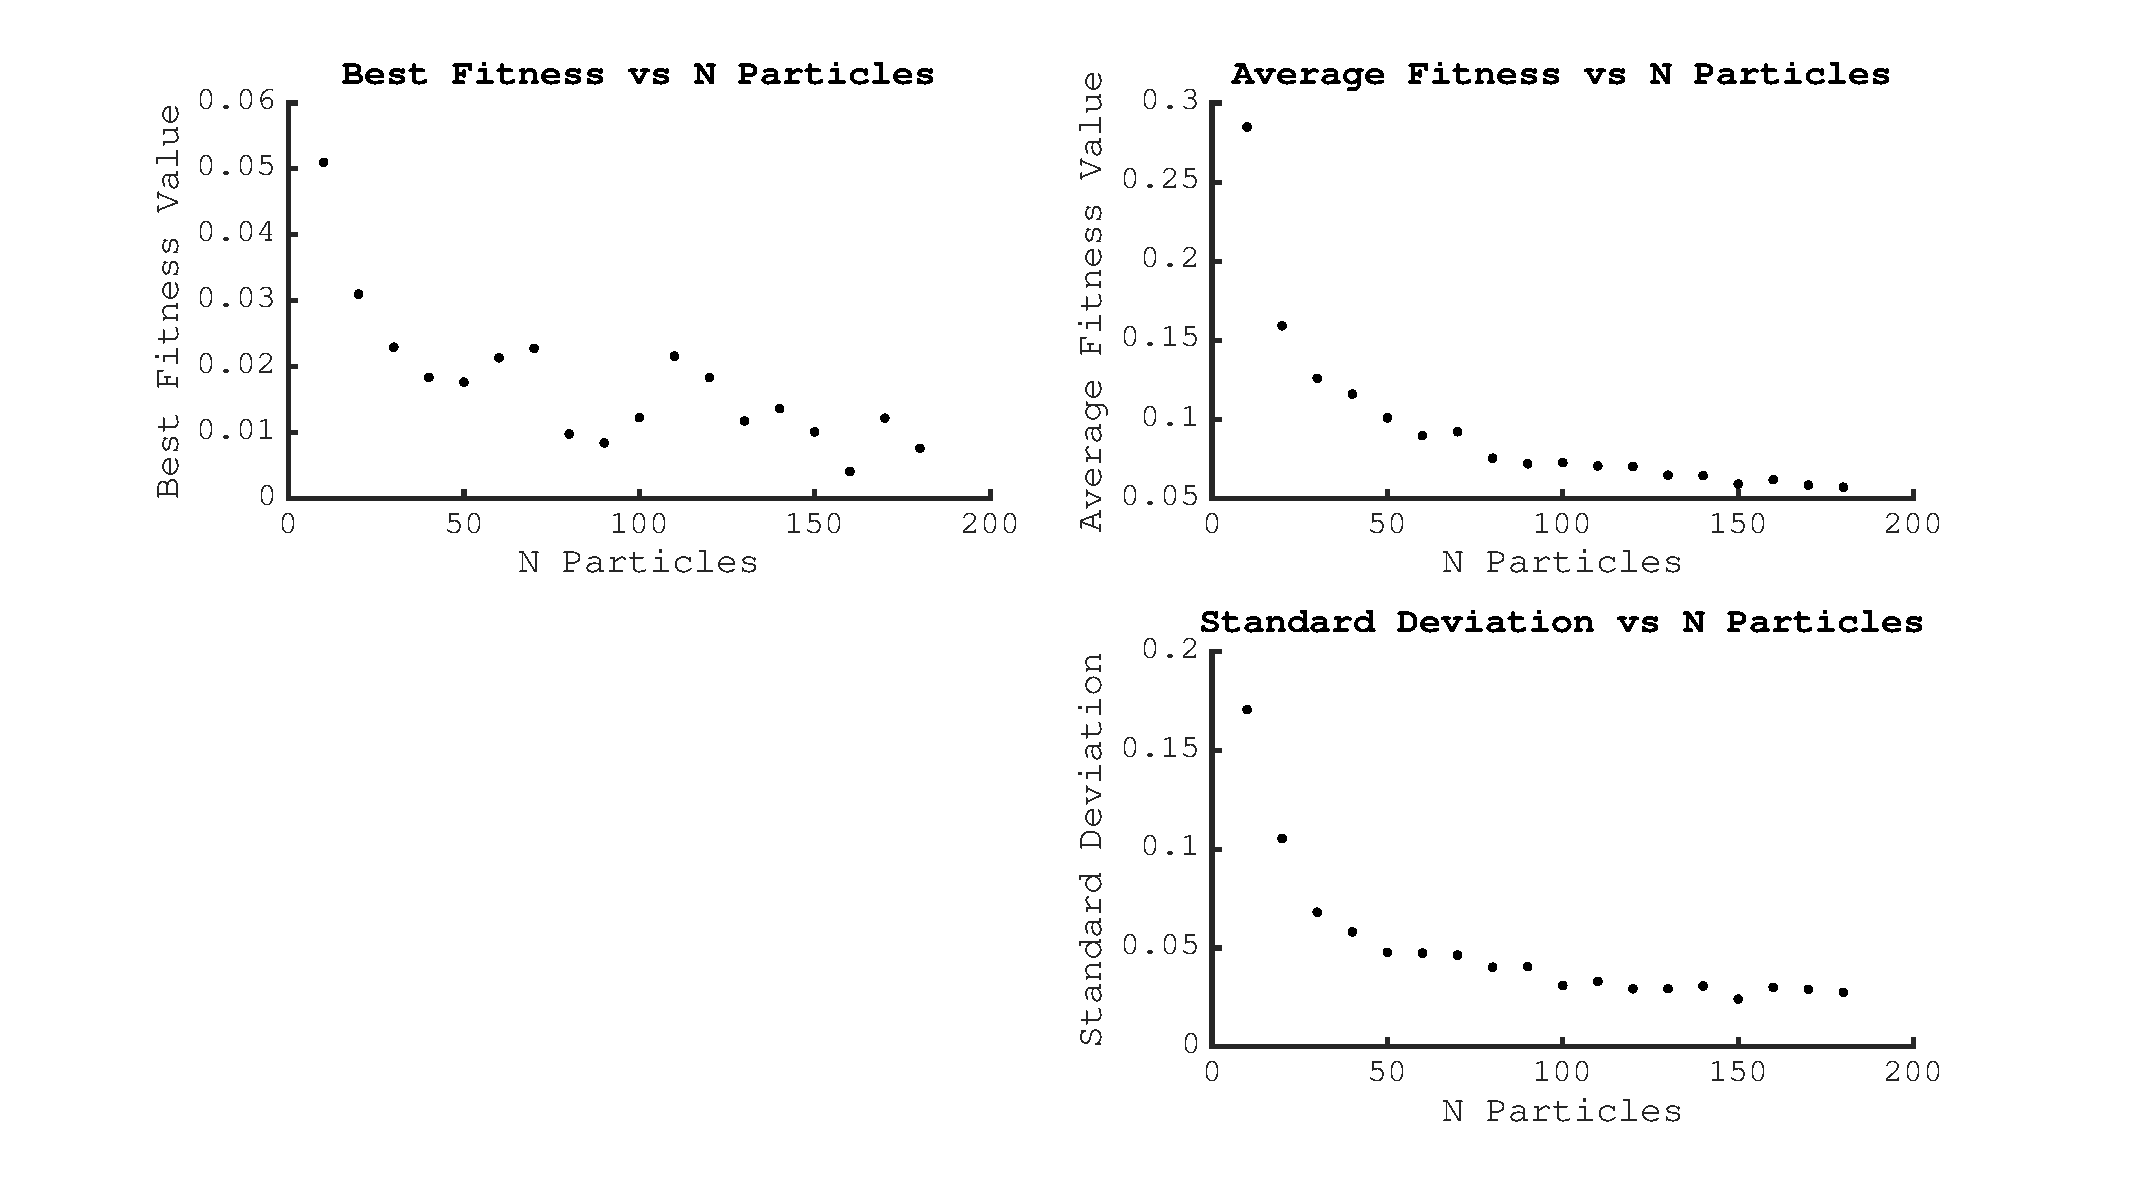
\includegraphics[width=0.93\textwidth]{particle_2d}
\caption{Best fitness, average, and standard deviation for various runs of varying number of particles.}
\label{fig:particle_2d}
\end{figure}

Using 72 trials, I then tested the \textit{crcbpso.m} function using multiple number of particles ranging from 10 to 180.
All other parameters were kept at default.
This time I also saved the best coordinate locations and plotted against number of particles used.
Figure \ref{fig:particle_2d} shows a clearly defined trend in the best fitness obtained.
Average fitness follows even more cleanly, and the standard deviation beautifully settles steadily past 100 particles used.
The best coordinates were also plotted in figure \ref{fig:particle_3d}.
Coordinate values also become smoother at 100 particles onwards.
Taking these results and computation time in mind, I decided to use 80 particles moving forwards.

The computation time ranged from 8 s at 10 particles, to 128.7 s at 180 particles.
Time increased by a factor of 0.7 s per particle added.
\pagebreak
\begin{figure}[h!]
\centering
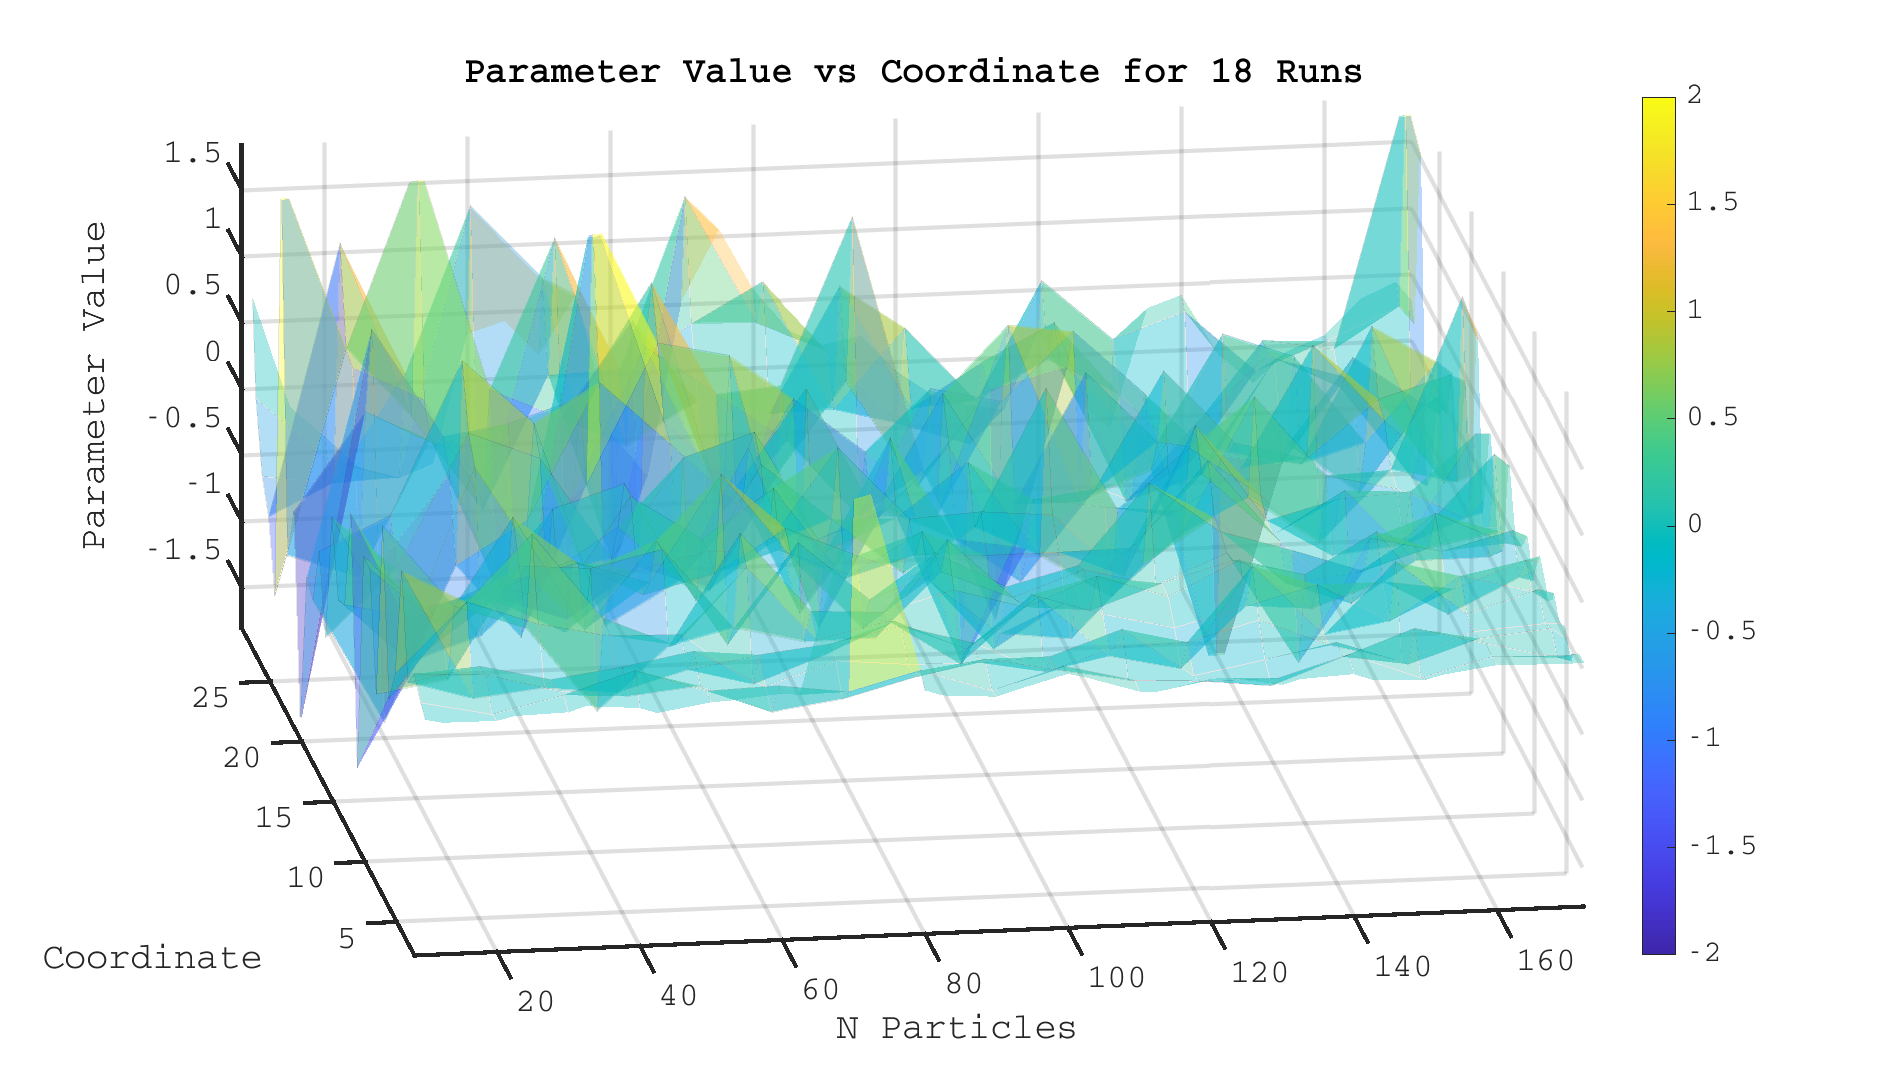
\includegraphics[width=0.65\linewidth]{particle_3d_1}
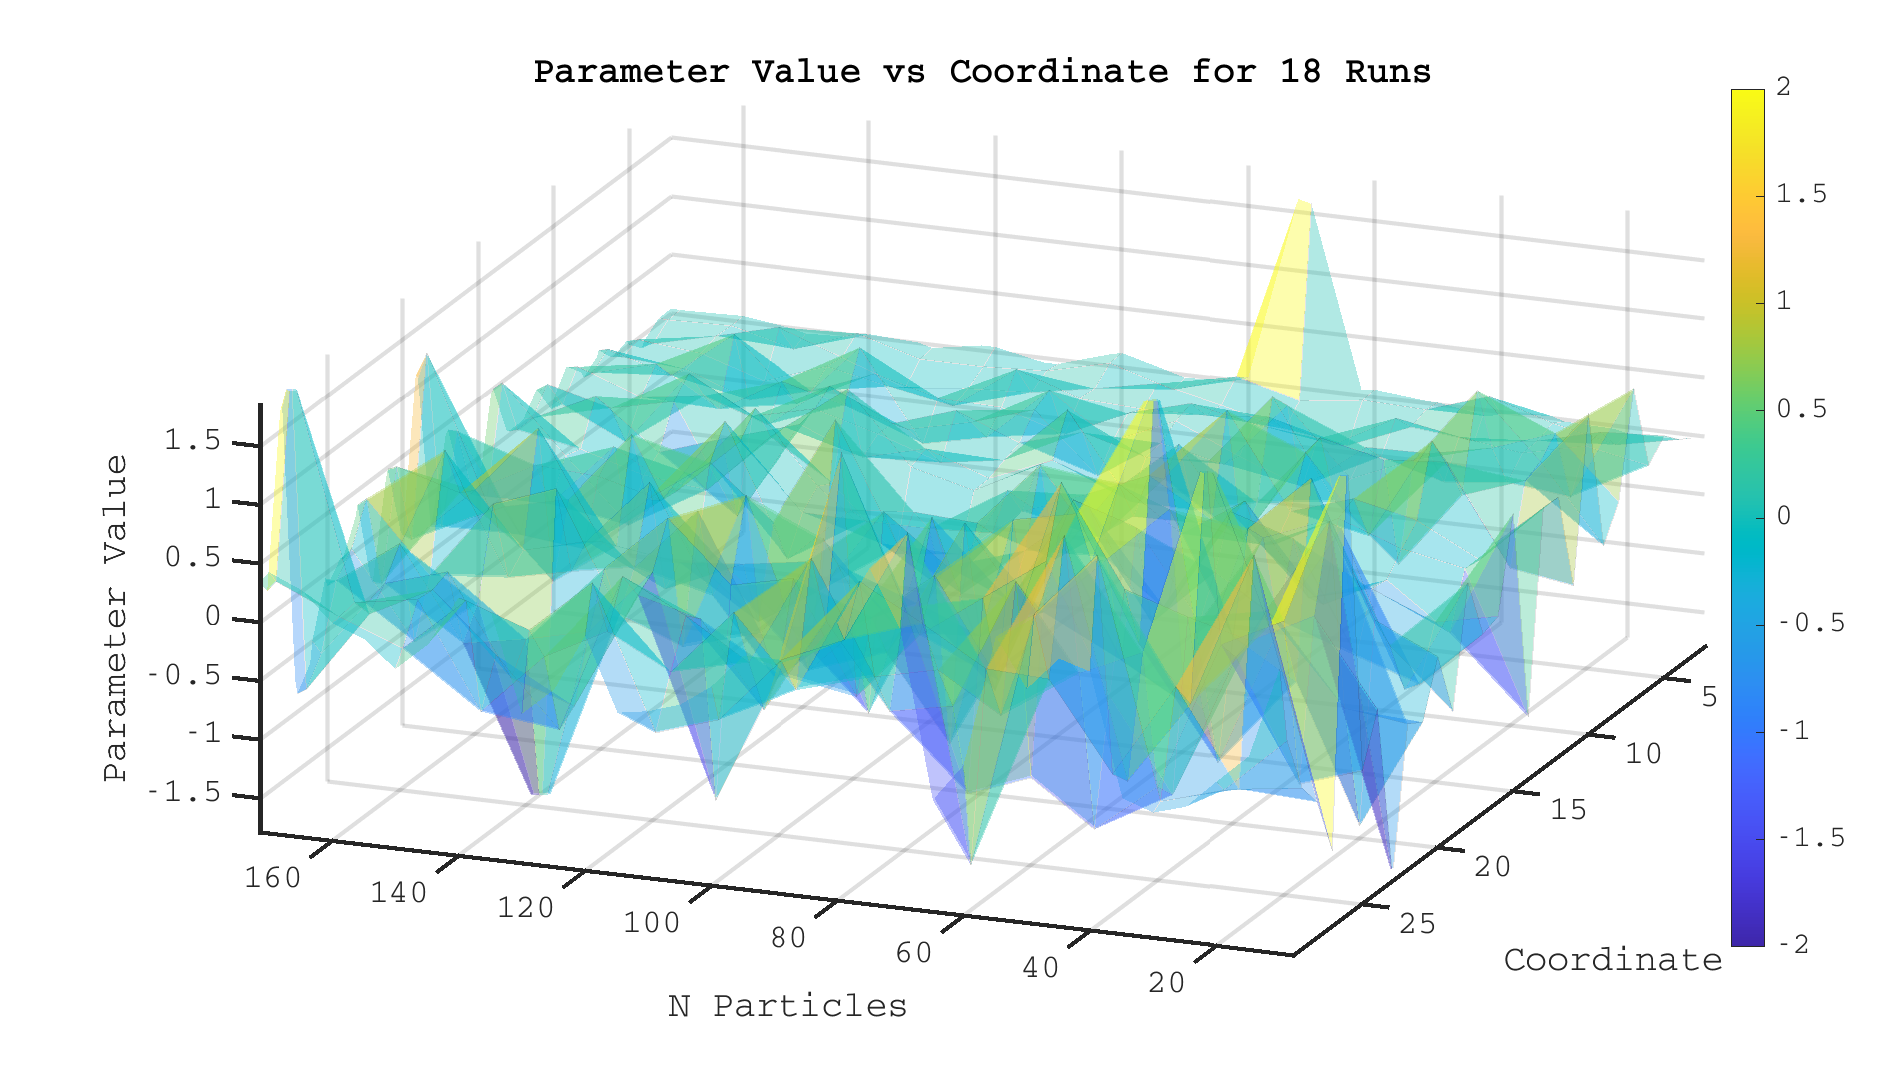
\includegraphics[width=0.65\linewidth]{particle_3d_2}
\caption{The value of each parameter as a function of number of particles used shown for each coordinate index.}
\label{fig:particle_3d}
\end{figure}

\subsection{Number of Steps}

Now using 72 trials and 80 particles, I varied the number of steps per \textit{crcbpso.m} computation.
I began at 750 steps increasing by 750 each new run.
It became evident instantly the number of steps governs the accuracy of the best fitness obtained more than any other tested parameter.
The best fit at 750 steps was 27.68, and by 2250 steps it was \(2.4\times10^{-4}\).
The same behavior is recognized in the 3d plot of coordinate sets in figure \ref{fig:steps_3d} as all coordinates approach 0.

\begin{figure}[h!]
\centering
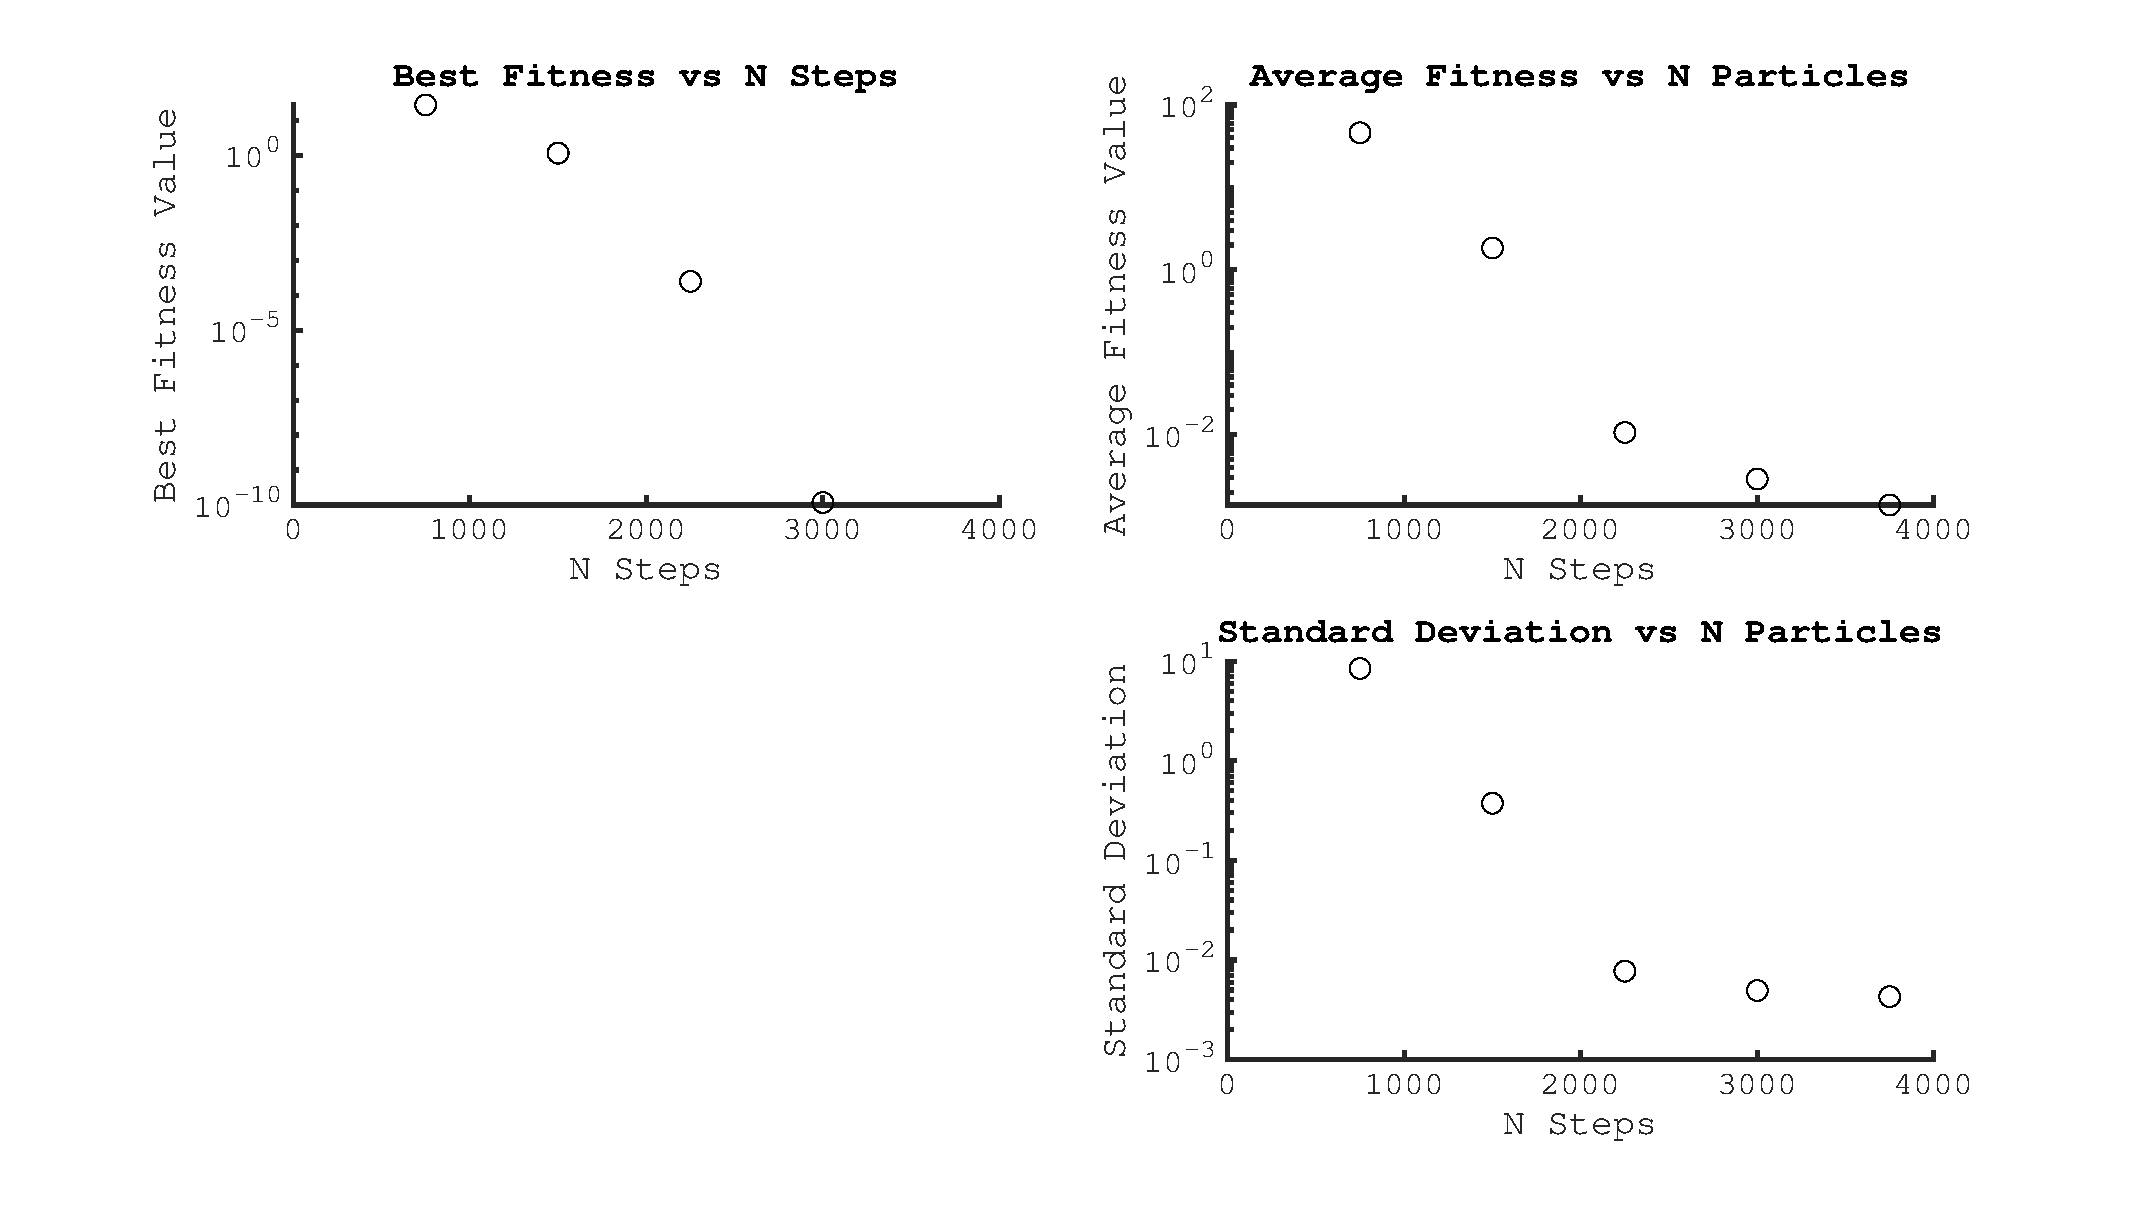
\includegraphics[width=0.93\textwidth]{steps_2d}
\caption{Best fitness, average, and standard deviation for various runs of varying number of steps.}
\label{fig:steps_2d}
\end{figure}

\begin{figure}[h!]
\centering
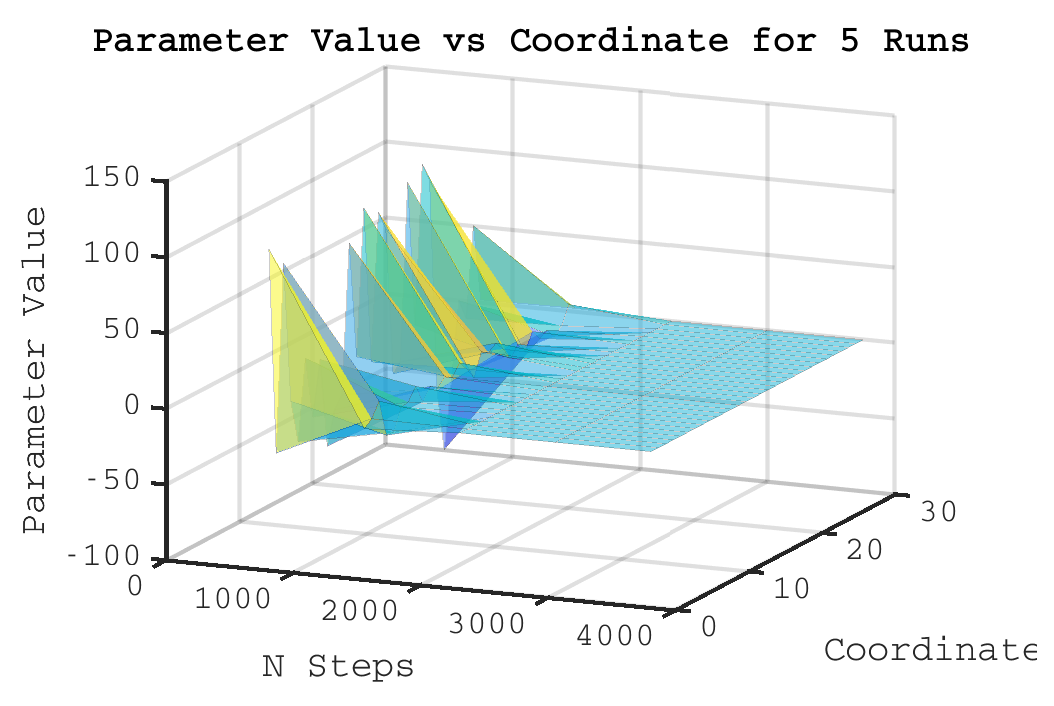
\includegraphics[width=0.73\textwidth]{steps_3d}
\caption{The value of each parameter vs number of steps shown for each coordinate index.}
\label{fig:steps_3d}
\end{figure}

\section{Conclusion}

This was an improvised approach at testing multiple ranges of parameters by taking advantage of short computation times through parallel processing.
Due to a lack of time, I resorted to eyeing approximately good parameter values, but a better approach is to least squares-fit my results to get more sound conclusions.
One could also change the order in which parameters are tested and compare multiple permutations. \\
\\
I believe the task of finding the optimal \textit{crcbpso.m} parameters is a PSO problem in itself. \\

\bibliographystyle{unsrt}
\bibliography{references}
\end{document}
